\chapter{Rapid Spanning Tree
Protocol}\label{rapid-spanning-tree-protocol}

\emph{COMPARISON OF STP VERSIONS (Standard vs.~Cisco)}

\begin{figure}
\centering
\pandocbounded{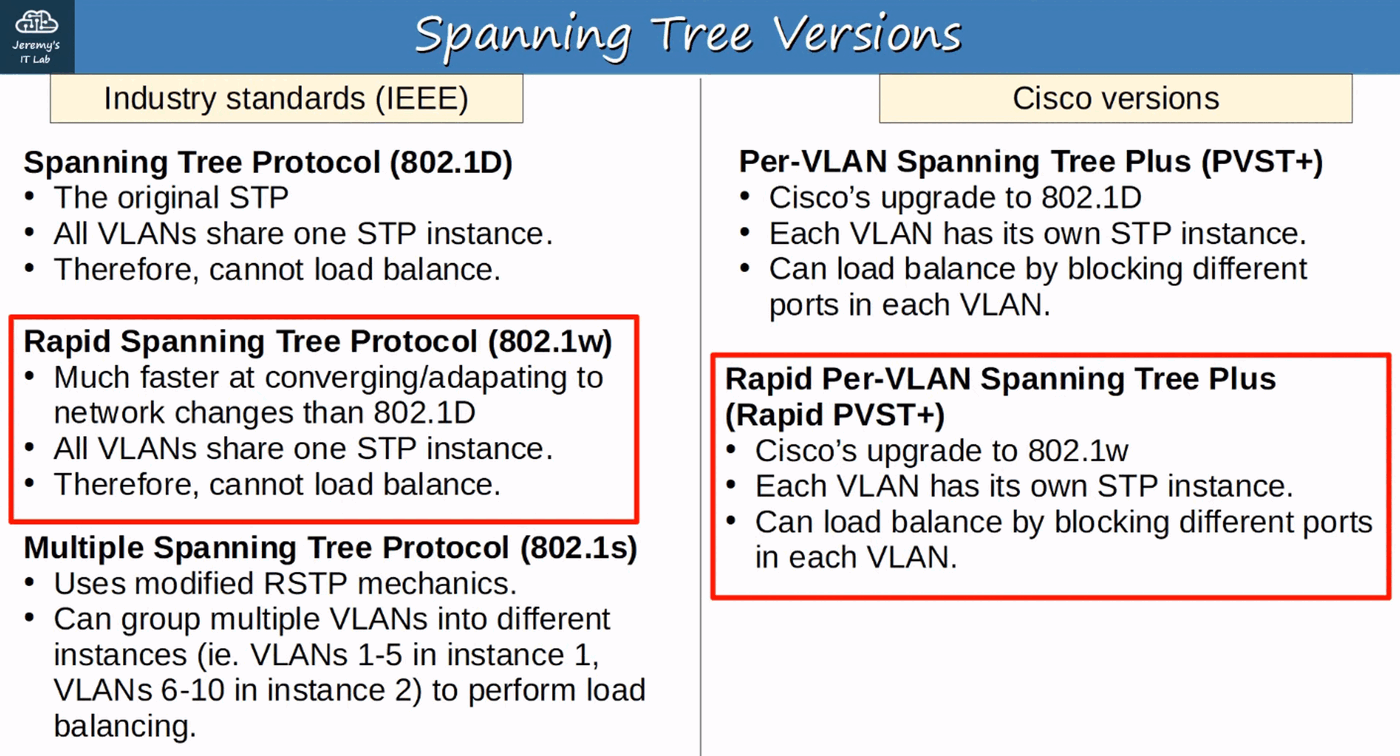
\includegraphics[keepaspectratio,alt={image}]{images/23-rapid-spanning-tree-protocol/img-001.png}}
\end{figure}

We are only concerned with 802.1w for MOST use cases.

MSTP (802.1s) is more useful for VERY LARGE networks.

WHAT IS RAPID PER-VLAN SPANNING TREE PLUS?

\begin{quote}
RSTP is not a time-based spanning tree algorithm like 802.1D. Therefore,
RSTP offers an improvment over teh 30 seconds or more 802.1D takes to
move a link to forwarding. The heart of the protocol is a new
bridge-bridge handshake mechanism, which allows ports to move directly
to forwarding
\end{quote}

\section{Similarities Between STP and
RSTP}\label{similarities-between-stp-and-rstp}

\begin{itemize}
\tightlist
\item
  RSTP serves the same purpose as STP, blocking specific PORTS to
  prevent LAYER 2 LOOPS.
\item
  RSTP elects a ROOT BRIDGE with the same rules as STP
\item
  RSTP elects ROOT PORTS with the same rules as STP
\item
  RSTP elects DESIGNATED PORTS with the same rules as STP
\end{itemize}

\section{Differences Between STP and
RSTP}\label{differences-between-stp-and-rstp}

\textbf{PORT COSTS}

\begin{figure}
\centering
\pandocbounded{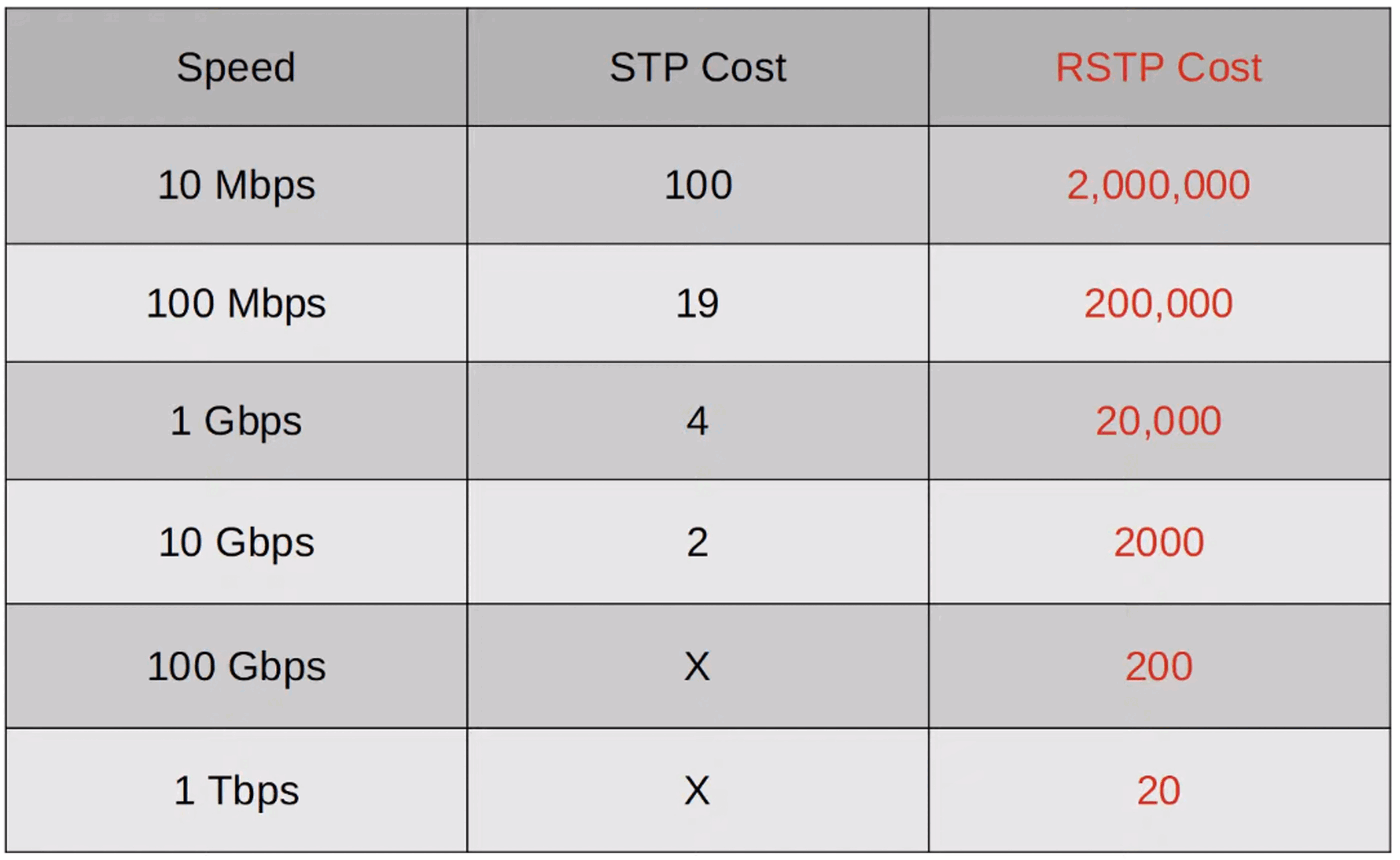
\includegraphics[keepaspectratio,alt={image}]{images/23-rapid-spanning-tree-protocol/img-002.png}}
\end{figure}

(STUDY AND MEMORIZE PORT COSTS OF STP AND RSTP)

\section{RSTP Port States}\label{rstp-port-states}

\begin{figure}
\centering
\pandocbounded{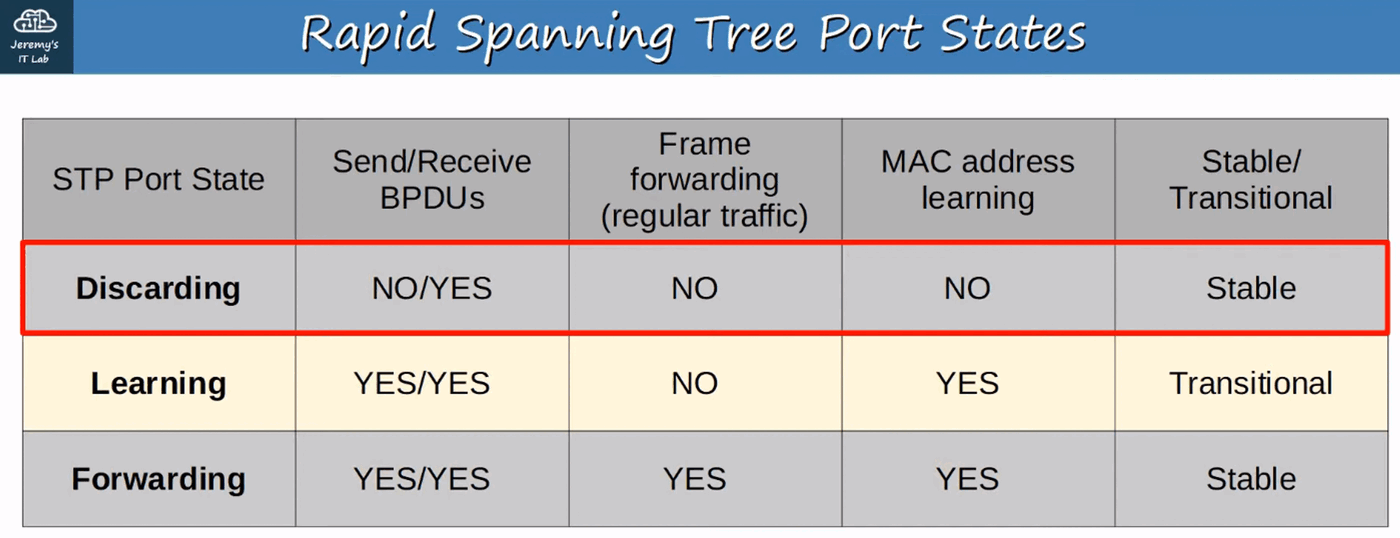
\includegraphics[keepaspectratio,alt={image}]{images/23-rapid-spanning-tree-protocol/img-003.png}}
\end{figure}

\begin{itemize}
\tightlist
\item
  If a PORT has been ADMINISTRATIVELY DISABLED (''shutdown'' command) =
  DISCARDING STATE
\item
  If a PORT is ENABLED but BLOCKING traffic to prevent LAYER 2 LOOPS =
  DISCARDING STATE
\end{itemize}

\section{RSTP Roles}\label{rstp-roles}

\begin{itemize}
\tightlist
\item
  The ROOT PORT role remains unchanged in RSTP

  \begin{itemize}
  \tightlist
  \item
    The PORT that is closest to the ROOT BRIDGE becomes the ROOT PORT
    for the SWITCH
  \item
    The ROOT BRIDGE is the only SWITCH that doesn't have a ROOT PORT
  \end{itemize}
\item
  The DESIGNATED PORT role remains unchanged in RSTP

  \begin{itemize}
  \tightlist
  \item
    The PORT on a segment (Collision Domain) that sends the best BPDU is
    that segment's DESIGNATED PORT (only one per segment!)
  \end{itemize}
\item
  The NON-DESIGNATED PORT role is split into TWO separate roles in RSTP:

  \begin{itemize}
  \tightlist
  \item
    The ALTERNATE PORT role
  \item
    The BACKUP PORT role
  \end{itemize}
\end{itemize}

\textbf{RSTP : ALTERNATE PORT ROLE}

\begin{itemize}
\tightlist
\item
  The RSTP ALTERNATE PORT ROLE is a DISCARDING PORT that receives a
  superior BPDU from another SWITCH
\item
  This is the same as what you've learned about BLOCKING PORTS in
  classic STP
\end{itemize}

\begin{figure}
\centering
\pandocbounded{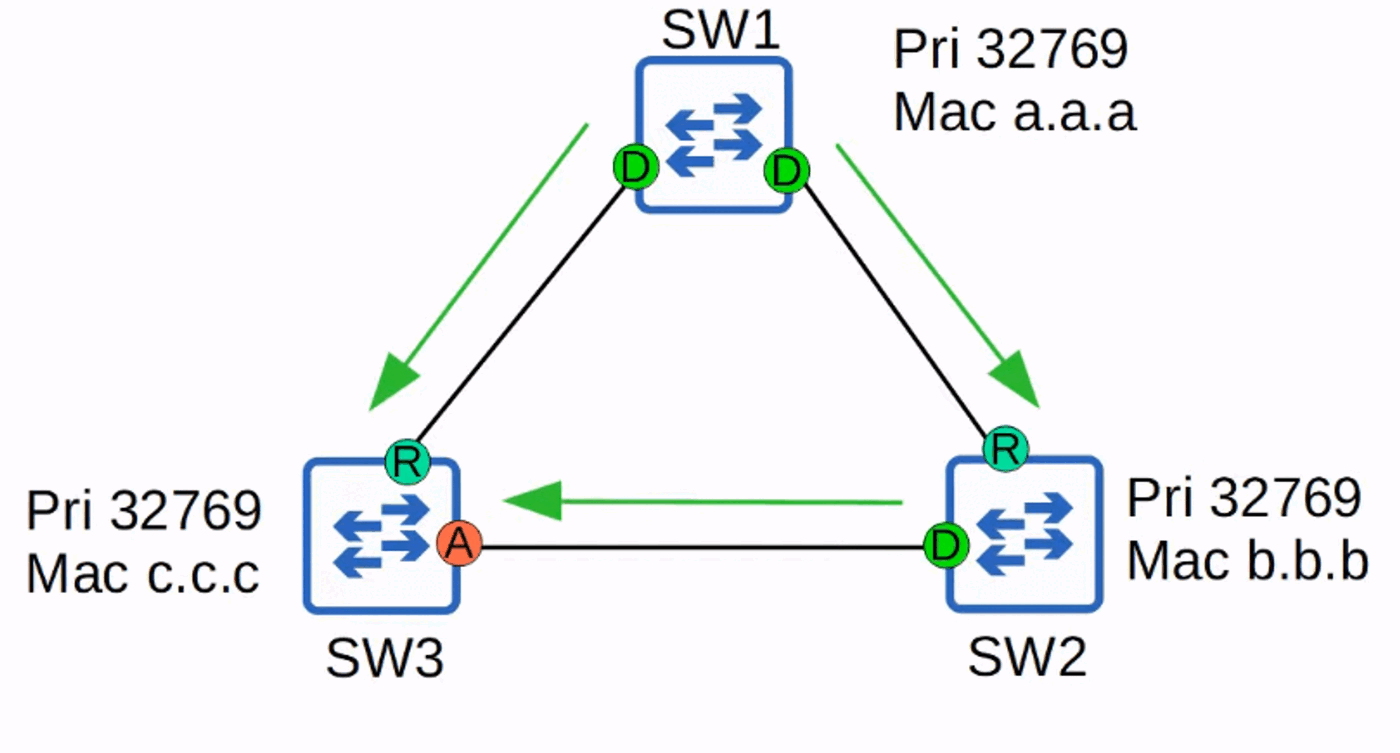
\includegraphics[keepaspectratio,alt={image}]{images/23-rapid-spanning-tree-protocol/img-004.png}}
\end{figure}

\begin{itemize}
\tightlist
\item
  An ALTERNATE PORT (labelled ``A'' above) functions as a backup to the
  ROOT PORT
\item
  If the ROOT PORT fails, the SWITCH can immediately move it's best
  alternate port to FORWARDING
\end{itemize}

\begin{figure}
\centering
\pandocbounded{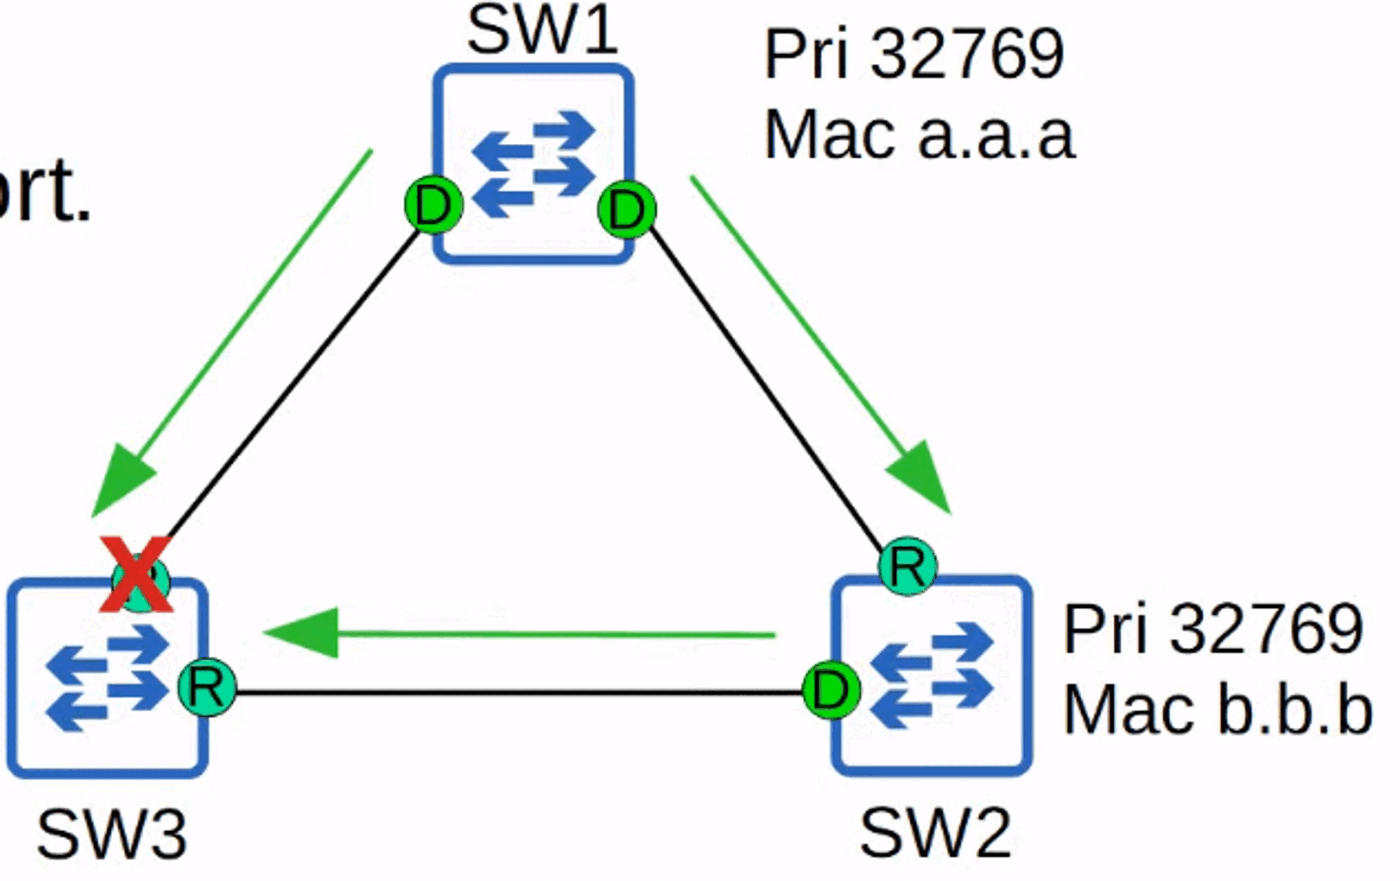
\includegraphics[keepaspectratio,alt={image}]{images/23-rapid-spanning-tree-protocol/img-005.png}}
\end{figure}

This immediate move to FORWARDING STATE functions like a classic STP
optional feature called \textbf{UplinkFast.} Because it is built into
RSTP, you do not need to activate UplinkFast when using RSTP/Rapid PVST+

One more STP optional feature that was built into RSTP is
\textbf{BackboneFast}

\begin{figure}
\centering
\pandocbounded{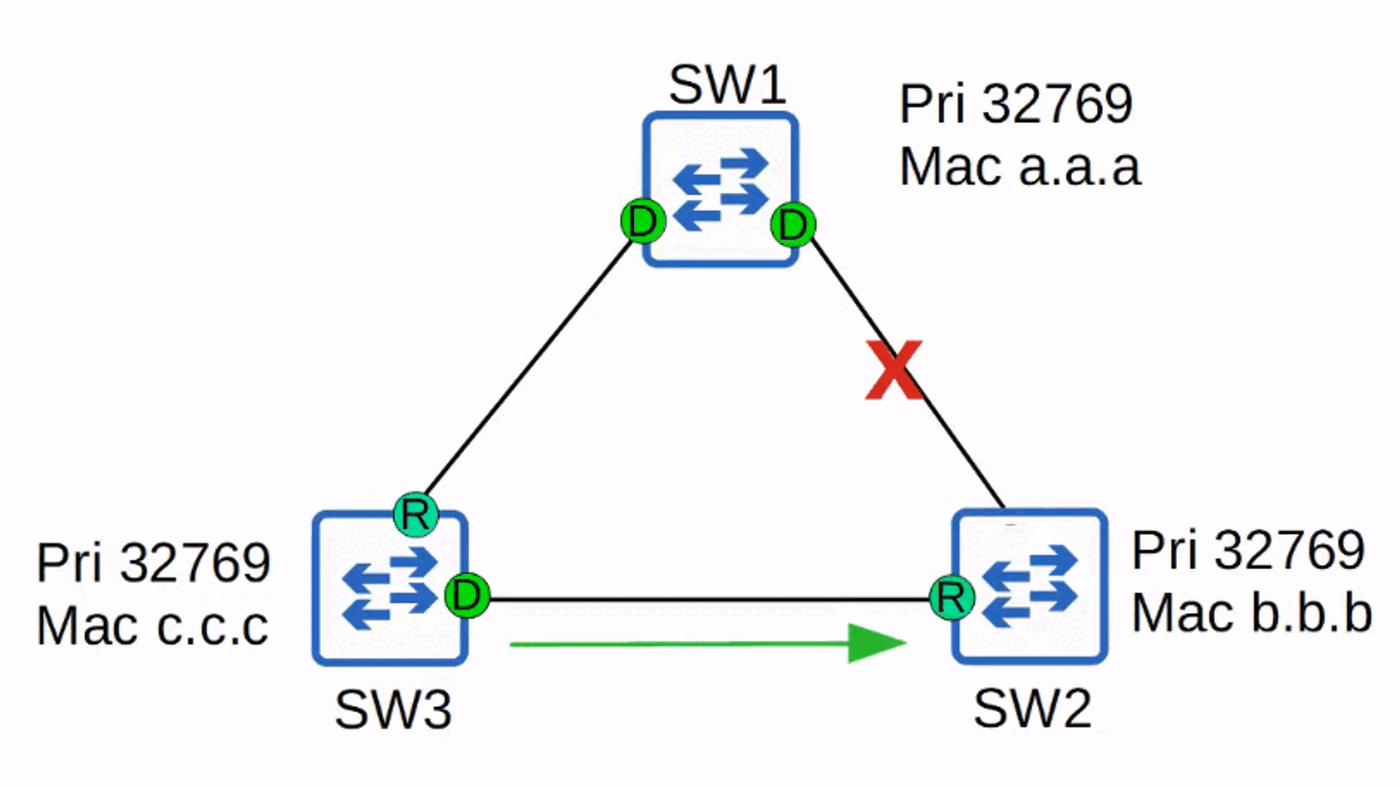
\includegraphics[keepaspectratio,alt={image}]{images/23-rapid-spanning-tree-protocol/img-006.png}}
\end{figure}

\begin{itemize}
\tightlist
\item
  \textbf{BackboneFast} allows SW3 to expire the MAX AGE TIMERS on it's
  INTERFACE and rapidly FORWARD the superior BPDUs to SW2
\item
  This FUNCTIONALITY is built into RSTP, so it does not need to be
  configured.
\end{itemize}

UPLINKFAST and BACKBONE FAST (SUMMARY)

\textbf{UplinkFast} and \textbf{BackboneFast} are two optional features
in Classic STP. They must be configured to operate on the SWITCH (not
necessary to know for the CCNA)

\begin{itemize}
\tightlist
\item
  Both features are built into RSTP, so you do NOT have to configure
  them. They operate, by DEFAULT
\item
  You do NOT need to have a detailed understanding of them for the CCNA.
  Know their names and their BASIC purpose (to help BLOCKING /
  DISCARDING PORTS rapidly move to FORWARDING)
\end{itemize}

\textbf{RSTP : BACKUP PORT ROLE}

\begin{itemize}
\tightlist
\item
  The RSTP BACKUP PORT role is a DISCARDING PORT that receives a
  superior BPDU from another INTERFACE on the same SWITCH
\item
  This only happens when TWO INTERFACES are connected to the SAME
  COLLISION DOMAIN (via a HUB)
\item
  Hubs are NOT used in modern networks, so you will probably NOT
  encounter an RSTP BACKUP PORT
\item
  Hubs are NOT used in modern networks, so you will probably NOT
  encounter an RSTP BACKUP PORT.
\item
  Functions as a BACKUP for a DESIGNATED PORT
\end{itemize}

The INTERFACE with the LOWERS PORT ID will be selected as the DESIGNATED
PORT, and the other will be the BACKUP port.

\begin{figure}
\centering
\pandocbounded{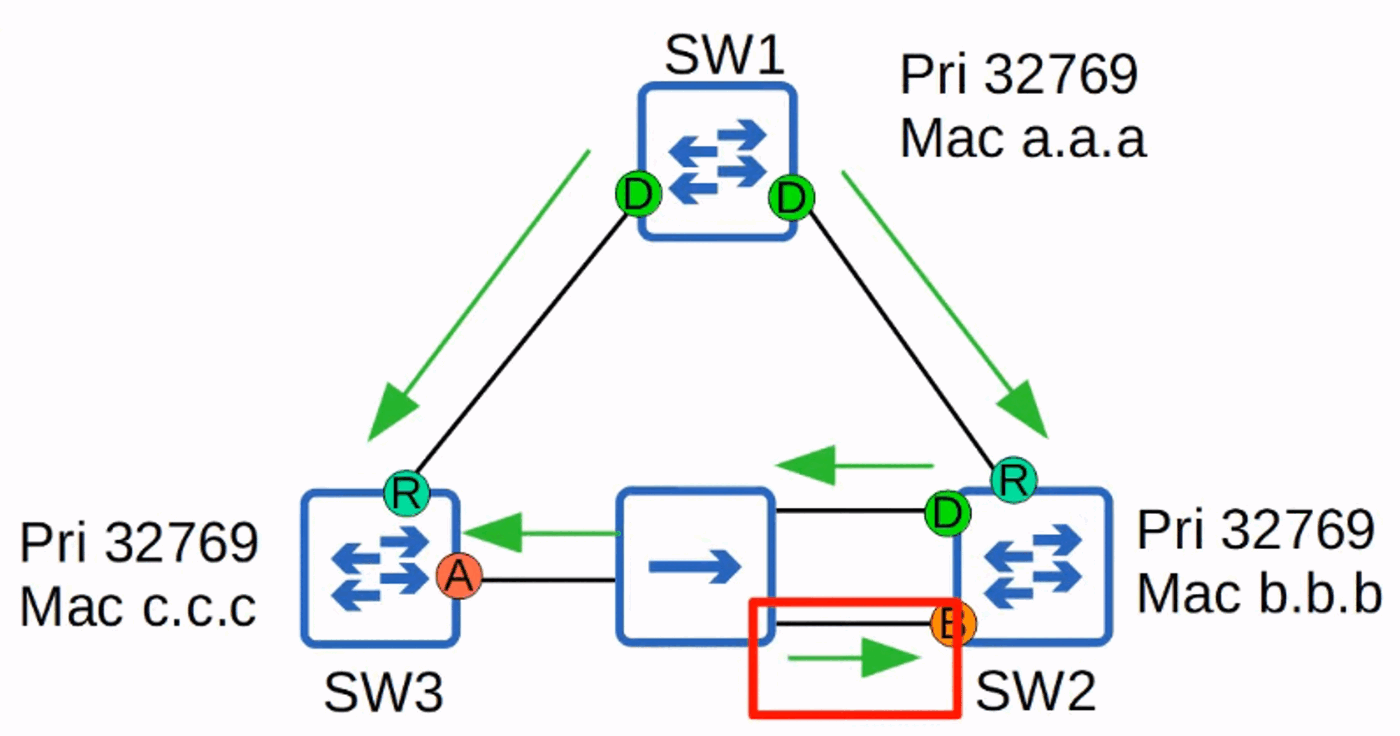
\includegraphics[keepaspectratio,alt={image}]{images/23-rapid-spanning-tree-protocol/img-007.png}}
\end{figure}

WHICH Switch will be ROOT BRIDGE? What about the OTHER ports ?

\begin{figure}
\centering
\pandocbounded{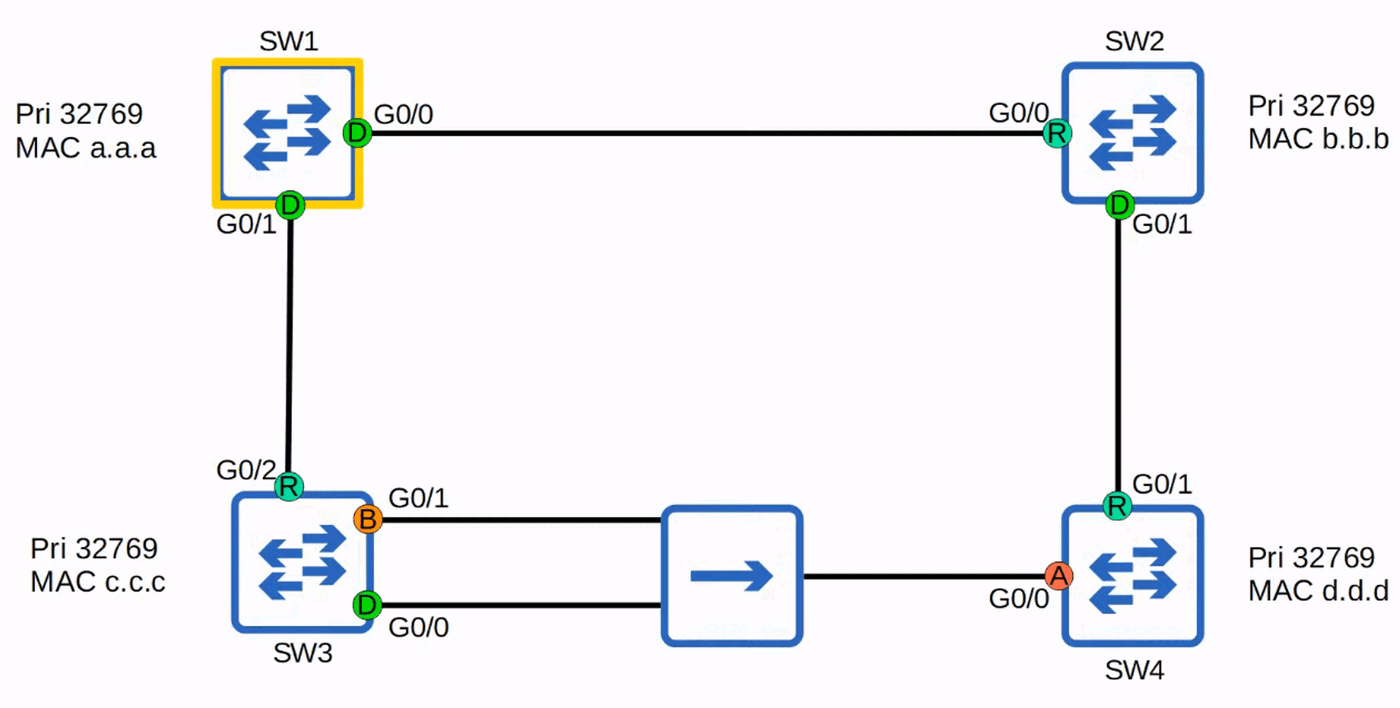
\includegraphics[keepaspectratio,alt={image}]{images/23-rapid-spanning-tree-protocol/img-008.png}}
\end{figure}

\begin{figure}
\centering
\pandocbounded{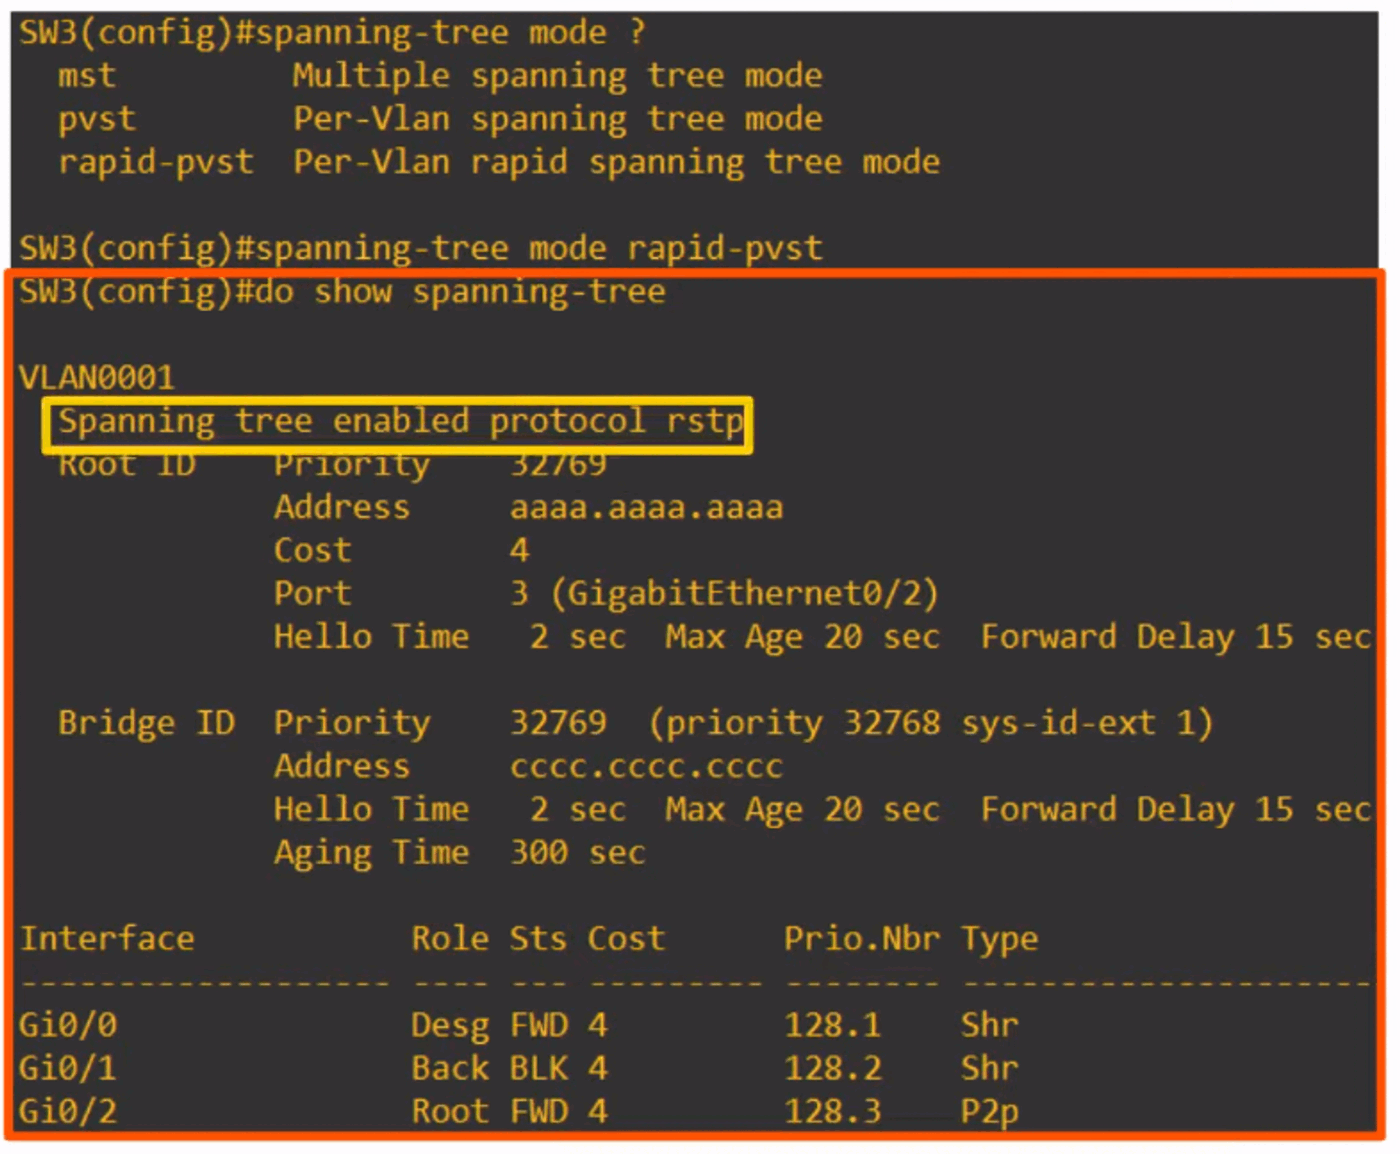
\includegraphics[keepaspectratio,alt={image}]{images/23-rapid-spanning-tree-protocol/img-009.png}}
\end{figure}

\begin{figure}
\centering
\pandocbounded{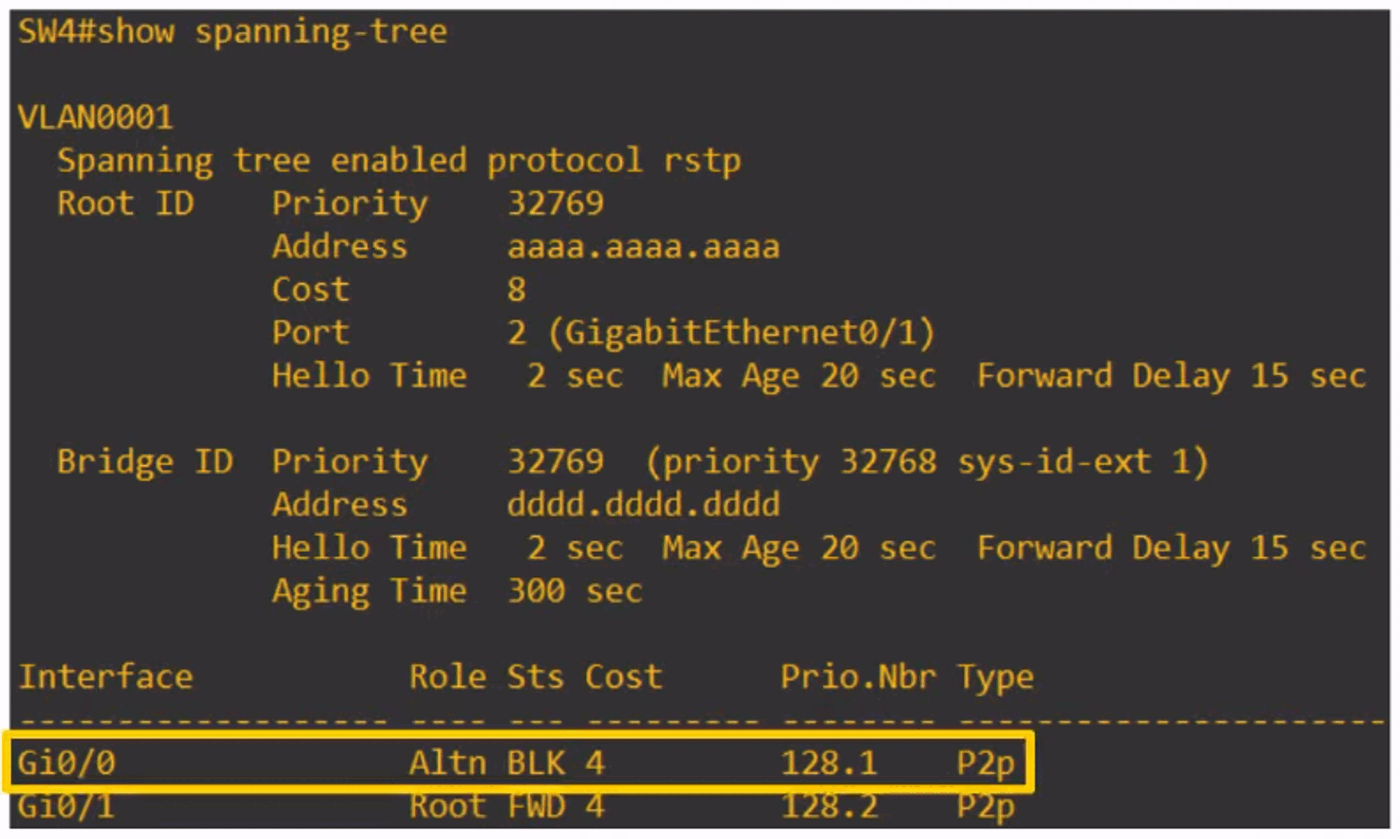
\includegraphics[keepaspectratio,alt={image}]{images/23-rapid-spanning-tree-protocol/img-010.png}}
\end{figure}

RAPID STP \emph{is} compatible with CLASSIC STP. The INTERFACE(S) on the
RAPID STP-enabled SWITCH connected to the CLASSIC STP-enabled SWITCH
will operate in CLASSIC STP MODE (Timers, BLOCKING
\textgreater\textgreater\textgreater{} LISTENING
\textgreater\textgreater\textgreater{} LEARNING
\textgreater\textgreater\textgreater{} FORWARDING, etc.)

\section{Rapid STP BPDU}\label{rapid-stp-bpdu}

CLASSIC RSTP (LEFT) vs RAPID STP BPDU (RIGHT)

\begin{figure}
\centering
\pandocbounded{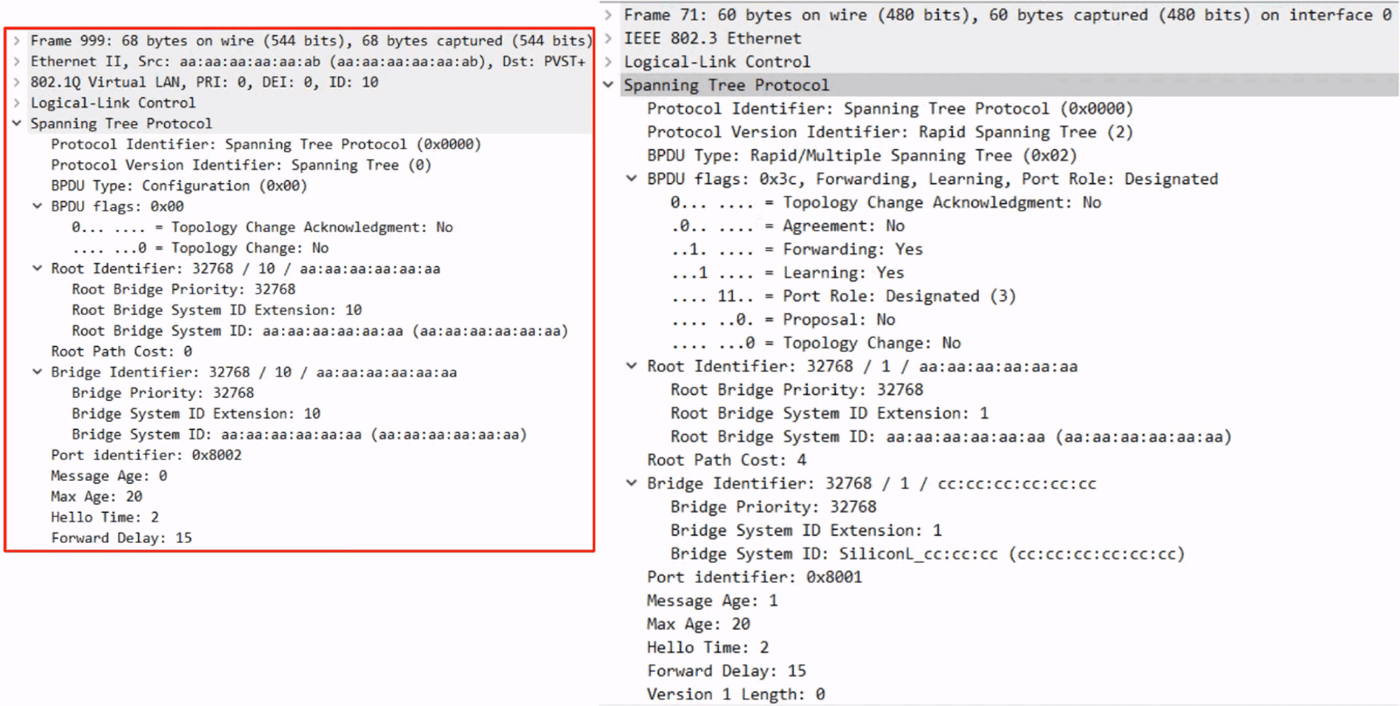
\includegraphics[keepaspectratio,alt={image}]{images/23-rapid-spanning-tree-protocol/img-011.png}}
\end{figure}

NOTE:

Classic STP BPDU has a ``Protocol Version Identifier: Spanning Tree (0)

BPDU Type: Configuration (0x00)

BPDU flags: 0x00

RAPID STP BPDU has a ``Protocol Version Identifier: Spanning Tree (2)

BPDU Type: Configuration (0x02)

BPDU flags: 0x3c

In CLASSIC STP, only the ROOT BRIDGE originated BPDUs, and other
SWITCHES just FORWARDED the BPDUs they received.

In RAPID STP, ALL SWITCHES originate and send their own BPDUs from their
DESIGNATED PORTS

\section{Rapid Spanning Tree
Protocol}\label{rapid-spanning-tree-protocol-1}

\begin{itemize}
\tightlist
\item
  ALL SWITCHES running RAPID STP send their own BPDUs every ``hello''
  time (2 Seconds)
\item
  SWITCHES ``age'' the BPDU information much more quickly

  \begin{itemize}
  \tightlist
  \item
    In CLASSIC STP, a SWITCH waits 10 ``hello'' intervals (20 seconds)
  \item
    In RAPID STP, a SWITCH considers a neighbour lost if it misses 3
    BPDUs (6 seconds). It will then ``flush'' ALL MAC ADDRESSES learned
    on that interface
  \end{itemize}
\end{itemize}

\begin{figure}
\centering
\pandocbounded{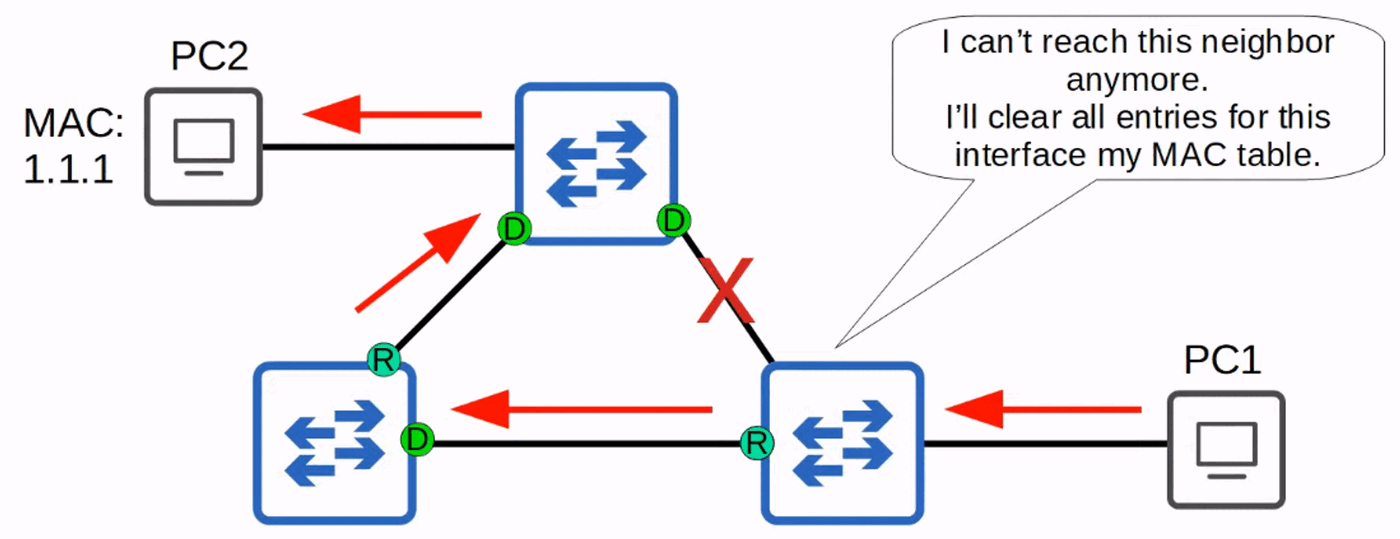
\includegraphics[keepaspectratio,alt={image}]{images/23-rapid-spanning-tree-protocol/img-012.png}}
\end{figure}

\section{RSTP Link Types}\label{rstp-link-types}

\begin{figure}
\centering
\pandocbounded{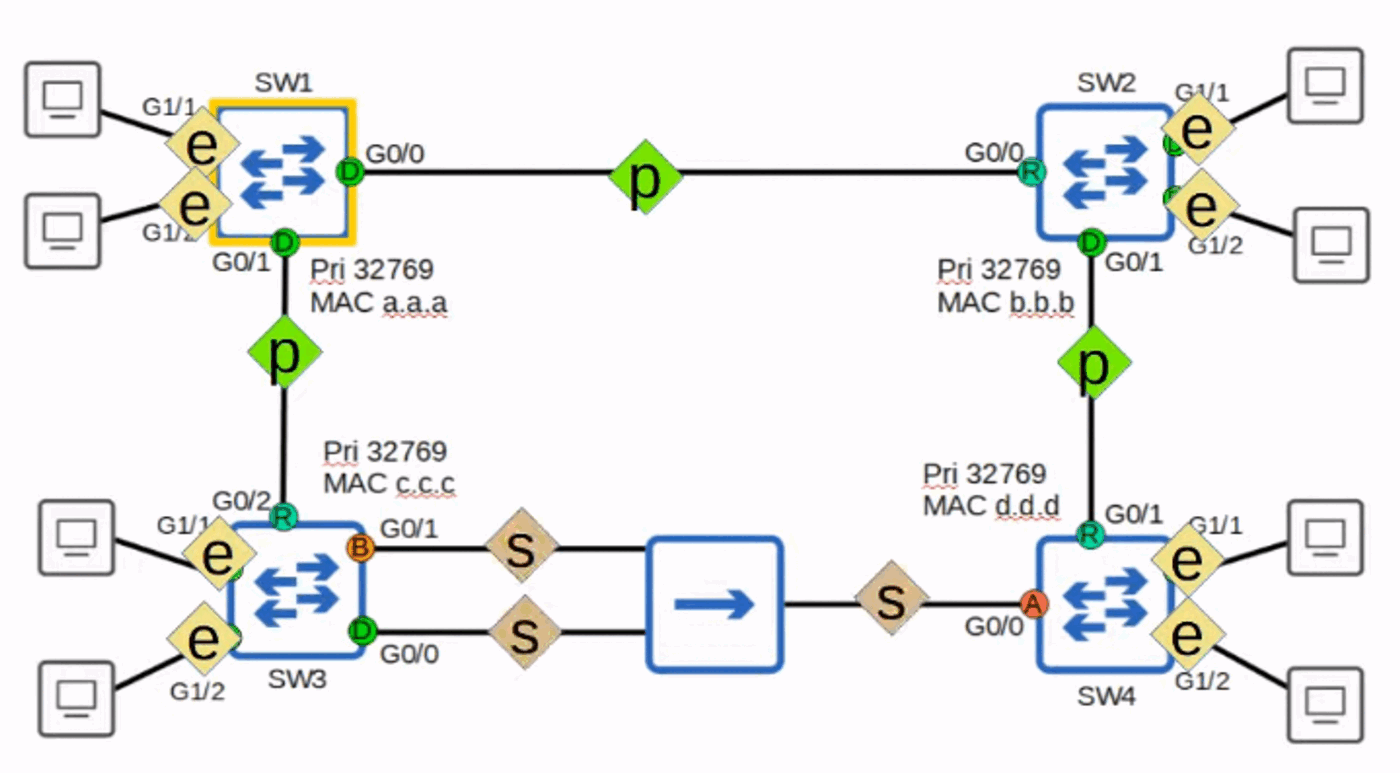
\includegraphics[keepaspectratio,alt={image}]{images/23-rapid-spanning-tree-protocol/img-013.png}}
\end{figure}

\begin{lstlisting}
<E> = EDGE

<P> = POINT-TO-POINT

<S> = SHARED
\end{lstlisting}

RSTP distinguishes between THREE different ``link types'' :
\textbf{EDGE}, \textbf{POINT-TO-POINT}, and \textbf{SHARED}

\section{Edge Ports}\label{edge-ports}

\begin{itemize}
\tightlist
\item
  Connected to END HOSTS
\item
  Because there is NO RISK of creating a LOOP, they can move straight to
  the FORWARDING STATE without the negotiation process!
\item
  They function like a CLASSIC STP PORT with PORTFAST ENABLED
\end{itemize}

SW1(config-if)\# spanning-tree portfast

\section{Point-to-Point Ports}\label{point-to-point-ports}

\begin{itemize}
\tightlist
\item
  Connect directly to another SWITCH
\item
  They function in FULL-DUPLEX
\item
  You don't need to configure the INTERFACE as POINT-TO-POINT (it should
  be detected)
\end{itemize}

SW1(config-if)\# spanning-tree link-type point-to-point

\section{Shared Ports}\label{shared-ports}

\begin{itemize}
\tightlist
\item
  Connect to another SWITCH (or SWITCHES) via a HUB
\item
  They function in HALF-DUPLEX
\item
  You don't need to configure the INTERFACE as SHARED (it should be
  detected)
\end{itemize}

SW1(config-if)\# spanning-tree link-type shared

\section{Quiz}\label{quiz}

\begin{figure}
\centering
\pandocbounded{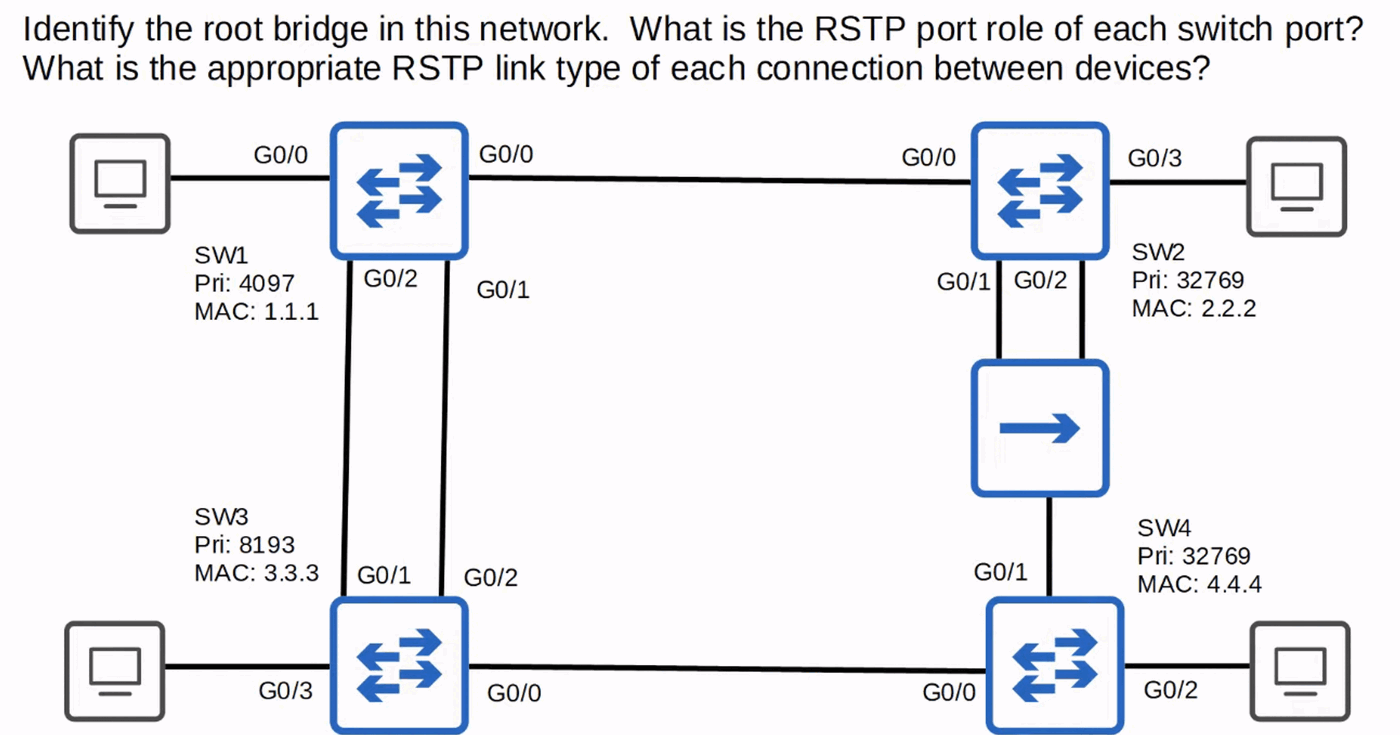
\includegraphics[keepaspectratio,alt={image}]{images/23-rapid-spanning-tree-protocol/img-014.png}}
\end{figure}

SW1 :

\begin{itemize}
\tightlist
\item
  \textbf{ROOT BRIDGE}
\item
  G0/0 - 0/3= DESIGNATED
\end{itemize}

SW2 :

\begin{itemize}
\tightlist
\item
  G0/0 = ROOT PORT
\item
  G0/1 = DESIGNATED PORT
\item
  G0/2 = BACKUP PORT
\item
  G0/3 = DESIGNATED PORT
\end{itemize}

SW3 :

\begin{itemize}
\tightlist
\item
  G0/0 = DESIGNATED PORT
\item
  G0/1 = ALTERNATE PORT
\item
  G0/2 = ROOT PORT
\item
  G0/3 = DESIGNATED PORT
\end{itemize}

SW4:

\begin{itemize}
\tightlist
\item
  G0/0 = ROOT
\item
  G0/1 = ALTERNATE PORT
\item
  G0/2 = DESIGNATED PORT
\end{itemize}

Connection between SW1 G0/0 and SW2 G0/0 = POINT-TO-POINT

Connection between SW3 G0/0 and SW4 G0/0 = POINT-TO-POINT

Connection between SW1 G0/1 and G0/2 to SW3 G0/1 and G0/2 =
POINT-TO-POINT

Connections to all the END HOSTS = EDGE

Connection from SW4 to HUB = SHARED

Connections from SW2 to HUB = SHARED

\section{Answer}\label{answer}

\begin{figure}
\centering
\pandocbounded{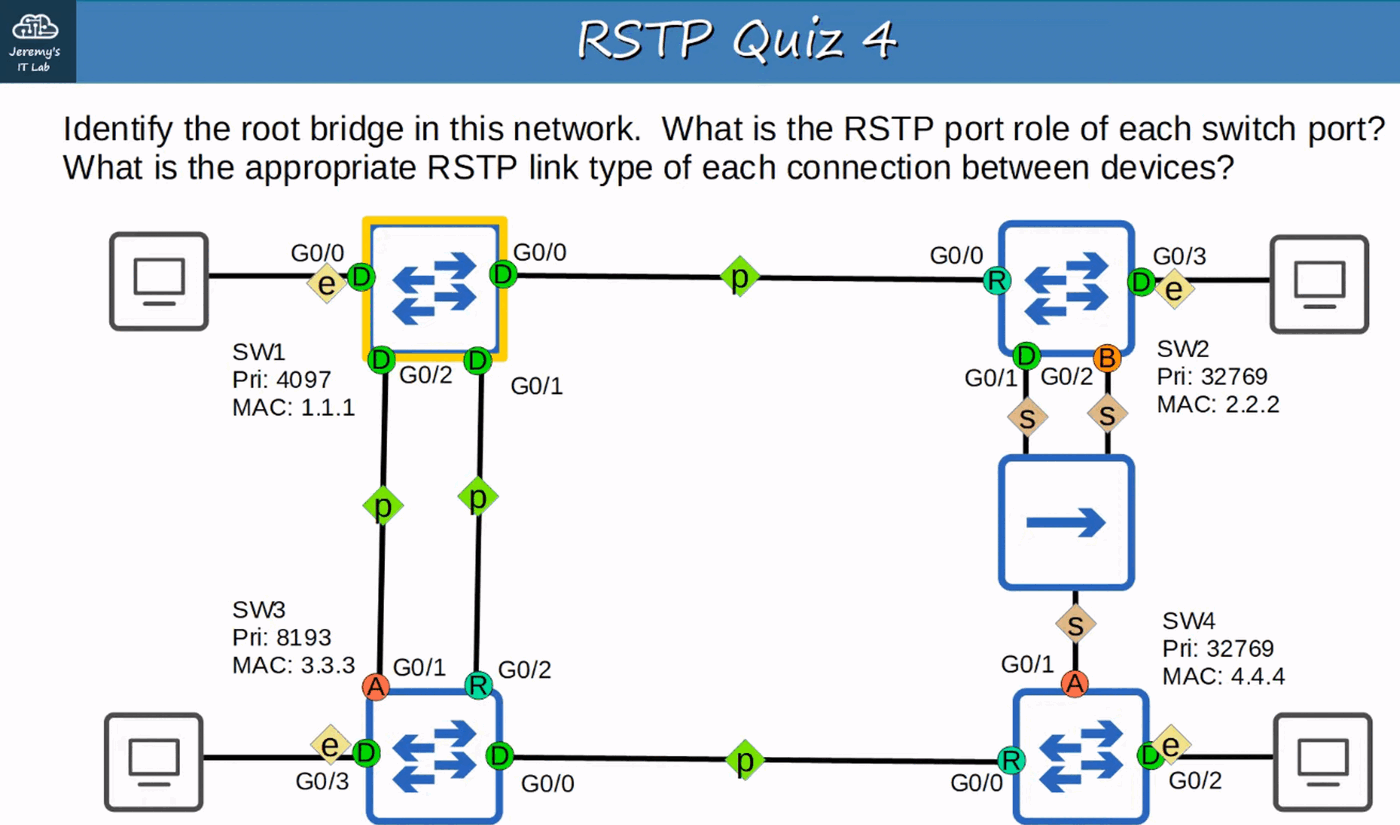
\includegraphics[keepaspectratio,alt={image}]{images/23-rapid-spanning-tree-protocol/img-015.png}}
\end{figure}
